\newcommand{\phsec}[1]{{\slshape #1}}
\chapter{Language Overview}
\label{chap:lang-overview}

\section{Introduction}

In this chapter we will provide you with the background knowledge you
need to understand \pharmml. We recommend that you read this chapter
before you work through the examples in chapter
\ref{chap:worked-egs}. The chapter will start by describing how a
\pharmml document is organised and then go on to illustrate some of
the key concepts and constructs of the language. For example, among
other things, we discuss variable and parameter scoping (section
\ref{sec:scoping-rules}), how to write maths (sections~\ref{sec:odes}
and~\ref{sec:maths}), and how to define data (section~\ref{sec:dataset}).
%and how to define and use units (section~\ref{sec:units}).
The chapter concludes with a discussion of the additional resources that
we expect to be used in support of \pharmml, but which are outside the
scope of this language specification (section~\ref{sec:supporting-res}).

\section{Organisation}
\label{sec:structure-overview}

As can be seen in figure \ref{fig:momloverview}, \pharmml is organised
into three main sections: \phsec{Model Definition}, \phsec{Trial
  Design} and \phsec{Modelling Steps}. This reflects the natural
organisation of a pharmacometric model and is the organisation
implicitly found in the M\&S tools used by modellers in this
area. Below we will go into more detail about the purpose and
organisation of each section.

% The
% \phsec{Model Definition} describes the model to be simulated, for
% which parameters are to be estimated, or which is to be analysed. The
% \phsec{Modelling Steps} section describes the process(es) used to
% simulate the model or estimate its parameters. Finally we have the
% \phsec{Trial Design} section. This describes the design of a clinical
% trial within \pharmml.

\begin{figure}[htb]
 \centering
  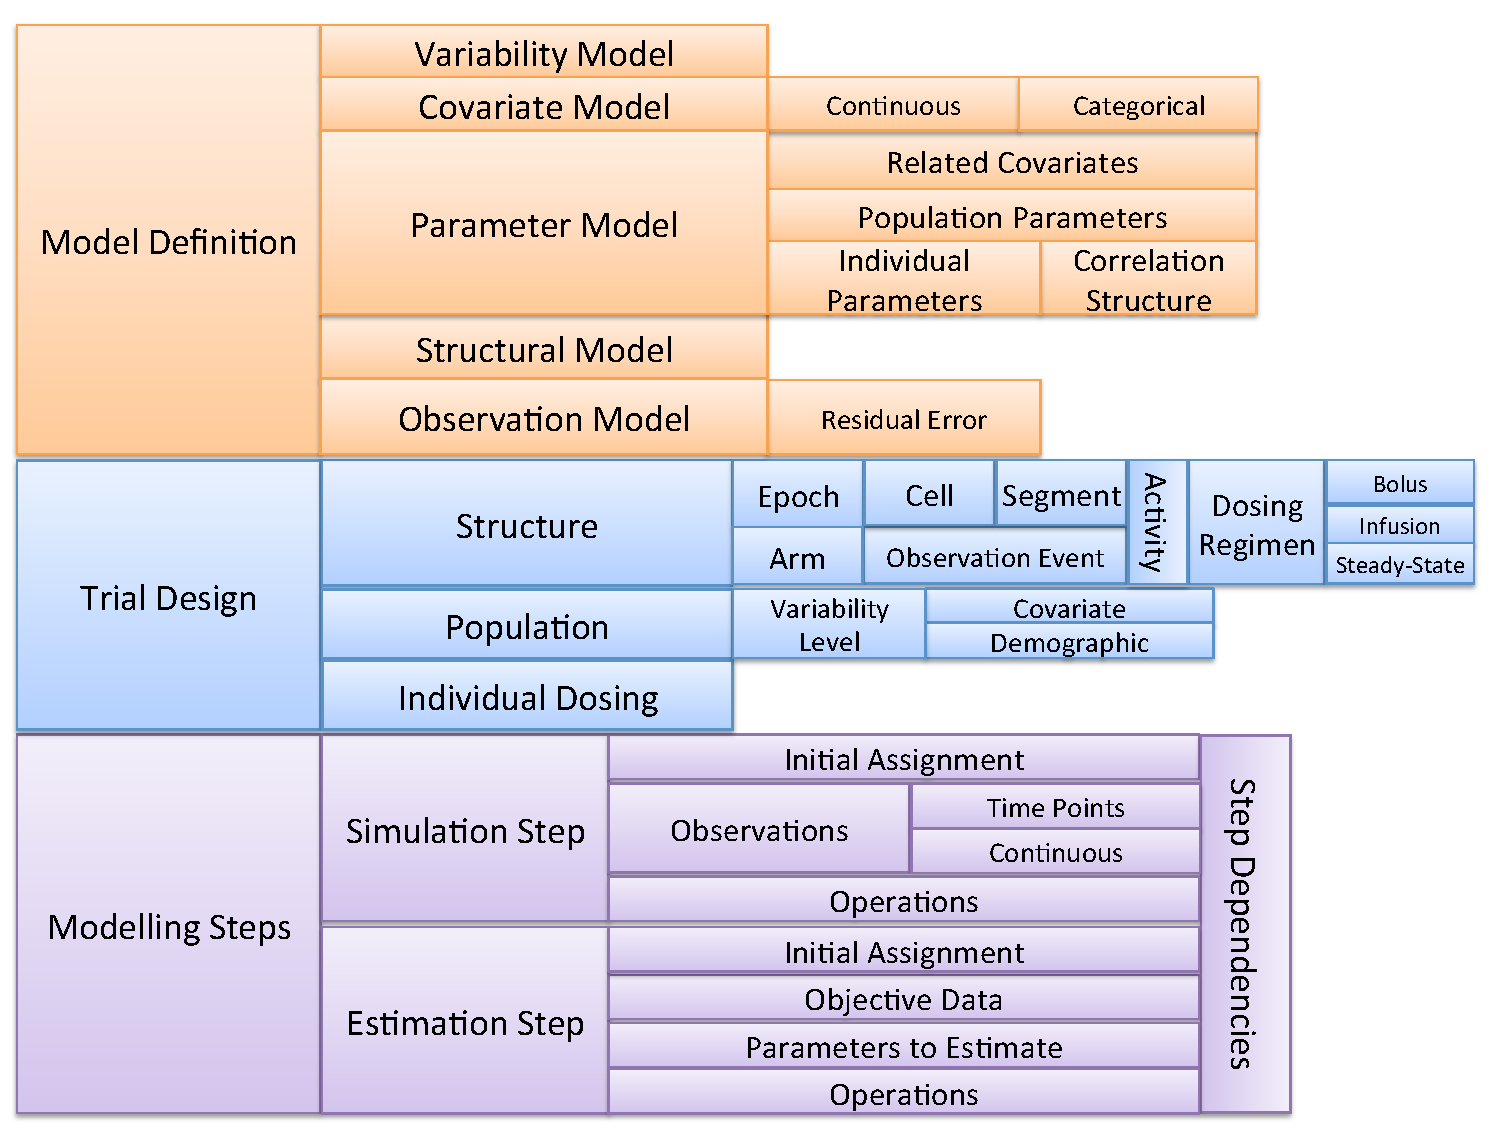
\includegraphics[height=0.4\textheight]{OverviewOfMoML}
  \caption{An overview of the organisation of \pharmml.}
  \label{fig:momloverview}
\end{figure}

% Below we will describe each section in more detail, but at this point it
% is worth noting that the \emph{minimal} \pharmml document describing a
% pharmacometric model must contain a \phsec{Model Definition}. It is
% also possible to describe a valid model with the \phsec{Model Definition} and
% \phsec{Trial Design}; and of course all three sections.

%Typically, this model could be reused in different
%scenarios and it is not necessarily specific to a particular clinical
%trial or simulation.

\subsection{Model Definition}

The \phsec{Model Definition} defines the model, typically a population
model, that describes the system under investigation and any variability
between individuals in the population. The modeller may wish to use
it for simulation, parameter estimation or other types of analysis and
exploration. The \phsec{Model Definition} in turn is composed of another
set of ``models'' that describe specific aspects of the overall model
definition. These are described below.

\subsubsection{Variability Model}
\label{sec:variability_model}

Variability is the concept that underpins a pharmacometric model and
the \phsec{Variability Model} enables us to describe this. Note that it
is possible to describe variability in a \pharmml model without
defining random variability, but by using covariates.
%\footnote{see Marc L.'s email [PUT URL HERE].}
Therefore the use of the \phsec{Variability Model}
is optional. In \pharmml you can use this to define
individual random variability, but also a hierarchy of variability
above and/or below the level of the individual (e.g.\xspace inter-occasion
variability). For more details of the theory behind the random
variability model, see section \ref{sec:variabilityModel}.


\subsubsection{Covariate Model}

The \phsec{Covariate Model} as you would expect from the name describes the
covariates used in the \phsec{Model Definition}. A covariate can be
continuous, in which case it is typically described by a continuous probability
distribution, or categorical. The formal description of the covariate
model can be found in section \ref{maths:covariate_model}.

\subsubsection{Parameter Model}

The \phsec{Parameter Model} principally describes the parameters of the model
definition and is typically used to describe parameters with some
level of variability (typically between subject variability). The
parameter is defined more formally in section
\ref{maths:parameter_defn}, but essentially for each parameter we
define a population term, one or more random effects, and its
relationship to the covariates defined in the covariate model. The
random effects can be defined at different levels of variability
(defined by the variability model, see section
\ref{sec:variability_model}), which includes capturing the correlation
between them --- essentially defining a covariance (or correlation)
matrix for each level of variability.

\subsubsection{Structural Model}

At the heart of the model definition are one or more \phsec{Structural
Model}s. These describe the system or systems that a modeller is
interested in and they represent a particular abstraction of that
system. For example a structural model may be used to describe the
pharmacokinetics of a drug. We can represent PK, PD or PK-PD models as
combinations of ODEs and algebraic equations.

\subsubsection{Observation Model}

In clinical trials experimental observations are made, and these
observations are subject to experimental error. Different types of
instrument, assay or material sampled will all have different
statistical errors associated with them. In a pharmacometric model
these errors are described using a residual error model (see
section~\ref{maths:error_model}). In \pharmml we encode the residual
error model using the \phsec{Observation Model}.

% The language permits the
% encoding of the more structured \emph{standard} and more flexible
% \emph{general} definition (this is described in more detail in
% section~\ref{maths:error_model}).

The outcomes of a clinical trial that we wish to model are not always
experimental measurements. A trial may aim to determine the efficacy
of an analgesic using a pain score provided by the subject; or measure
the frequency of seizure based on the maximum drug concentration; or
establish the remission rate over a given time in a cancer trial
\cite{Bonate:2011fk}. In each of these cases one needs to use a
discrete statistical model to represent these outcomes. These will
also be defined in the Observation Model, but at the moment are not
supported by the current version of \pharmml (see chapter
\ref{chap:scope}).

\subsection{Trial Design}

Clinical trials are carefully structured and can vary considerably in
their complexity. Typically, a trial will be structured into one or
more groups with each group subject to one or more treatment regimens
and observation protocols. Each group is then populated with individuals
from a population of subjects who have been screened for their
suitability to participate in the trial. In \pharmml we describe
the structure and population of a trial
explicitly in a dedicated section. This differs from some other
approaches, bit we feel it makes the clinical trial much clearer to
document and easier to encode computationally. More information can be
found in chapter~\ref{sec:CTS}.

% Typically in tools such as NONMEM and MONOLIX, the trial design is
% encoded within a tabular data-file. This file contains the dosing
% information, covariates and the experimental observations of each
% individual in the trial. In addition the definition of the structure
% of the clinical trial is also embedded in this table too. Clearly the
% data-file contains a lot of redundant information.

% In \pharmml we separate this information into the following three
% classes\footnote{It is interesting to note that the developers of
%   PharML had a similar insight and organised data in a similar
%   way\cite{NLMEcons:2008}.}:
% %
% \begin{description}
% \item[Population] The attributes of the individuals in the study: the
%   population in the population model. Each individual has a weight,
%   an age, a gender and numerous other properties that may or may not
%   be modelled as covariates in a given model. In addition, these
%   properties may change over time.
% \item[Dosing] When and how a drug or drugs are administered to the
%   individuals in the trial.
% \item[Measurements] These are the observations taken from each
%   individual and specific times during the study. Such measurements
%   provide the observations used during parameter estimation and are
%   typically the outputs calculated during a simulation.
% \end{description}
% %
% By separating out these classes of information you can see that the
% information we need to define the clinical trial is as follows:
% %
% \begin{description}
% \item[Trial Structure] The organisation of the trial, how the subjects
%   are grouped into different treatment groups and what the dosing
%   regiment is within these treatment groups.
% \item[Population] As above, the properties specific to the individual,
%   including those that vary over time.
% \item[Individual Dosing] This is related to the treatment regimens
%   described in the trial structure, but describes the dosing of each
%   subject in the study.
% \end{description}
% %
% The measurement data is then used exclusively for estimation.

% \begin{figure}[htb]
% \centering
% 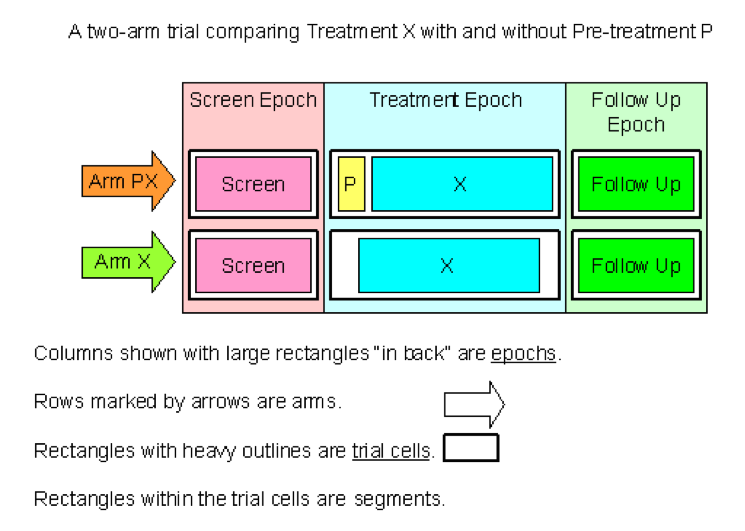
\includegraphics[height=0.35\textheight,clip=true,trim=0 0.5cm 0 0]{change_proposals/CDISCTrialStructure}%
% \caption{Overview of the Trial Structure used in the CDISC Study
%   Design Model.}
% \label{fig:cdiscstruct}
% \end{figure}

%  To define the Trial Structure we have reused, almost verbatim, the
% CDISC Study Design Model\footnote{CDISC URL to go here.}, which is an
% XML representation of a clinical trial. The figure below (figure
% \ref{fig:cdiscstruct}) shows how the CDISC trial structure is
% organised. It has five main components:
% \begin{description}
% \item[Epoch] The epoch defines a period of time during the study which
%   has a purpose within the study. For example a washout or a treatment
%   window. In CDISC Epochs can describe screening or follow-up periods,
%   which are out of the scope of \pharmml. An epoch is usually defined
%   by a time period.
% \item[Arm] The arm represents a path through the study taken by a
%   subject. An arm is composed of a study cell for each epoch in the study.
% \item[Cell] The study cell describes what is carried out during an
%   epoch in a particular arm. There is only one cell per epoch.
% \item[Segment] The segment describes a set of planned observations and
%   interventions, which may or may not involve treatment. Note that in
%   \pharmml our definition is more limited and we only describe
%   treatments. A segment can contains one or more activities.
% \item[Activity] The activity is an action that is taken in the
%   study. Here it is typically a treatment regimen.
% \item[StudyEvent] A study event describes the collection of
%   information about a particular individual. In CDISC this can be
%   information captured during screening or other non-treatment phases
%   of the clinical trial. But here we restrict it to capturing
%   observations during the treatment. In \pharmml this is how we
%   capture occasions.
% \end{description}
%  %
% Using this design gives us the reassurance that \pharmml will be able
% to represent all trial structures that we are likely to encounter.

% Examples of how a trial design is encoded in \pharmml can be found in
% the examples (chapter~\ref{chap:worked-egs}).


\subsection{Modelling Steps}
\label{sec:stepdeps}
The final element when describing an M\&S experiment, after defining
the model and the associated trial design, is to describe how the
model was used. This section of a \pharmml document is akin to the
Methods section of a paper. The aim is not to replicate your modelling
exactly, but to provide enough information to reproduce the
model\footnote{To replicate the execution of a model requires detailed
  information about not only what algorithms were used to simulate or
  execute a model, but also what software implementation was used and
  exact supporting libraries such as that of the random number
  generator.}.

\section{Identifiers, references and namespaces}

In \pharmml we use the Object Identifier to identify components in the
\phsec{Trial Design} and \phsec{Modelling Steps} sections of a \pharmml document and
the Symbol Identifier to identify parameters and variables within the
\phsec{Model Definition} section. Below we will describe the rules associated
with how they are defined and referenced.


\subsection{Object identifiers}

The concept of the Object Identifier is borrowed from the CDISC XML
description of a trial design \cite{CDISC:2011a}. There they use the
attribute \xatt{oid} to identify and to reference components used in
the design. Object identifiers have global scope, which means that all
object identifiers defined in a \pharmml document must be unique.

Elements that reference an object identifier by convention use the
attribute \texttt{oidRef} and the id referred to must exist in the
\pharmml document. In addition the object referred to must be
compatible with the element referencing it. The example below shows
how this works:
%
\begin{xmlcode}
<Epoch oid="e1">
  <!-- Detail omitted -->
</Epoch>
<Arm oid="a2">
  <!-- Detail omitted -->
</Arm>
<Cell oid="c2">
    <EpochRef oidRef="e1" />
    <ArmRef oidRef="a2"/>
    <SegmentRef oidRef="tb"/>
</Cell>
\end{xmlcode}
%
Here the element \xelem{EpochRef} refers to the object identifier of
the Epoch, ``e1'', and the \xelem{ArmRef} element refers to the Arm
object, ``a2''. This is correct. However, the following example
is incorrect:
%
\begin{xmlcode}
<Epoch oid="e1">
  <!-- Detail omitted -->
</Epoch>
<Arm oid="a2">
  <!-- Detail omitted -->
</Arm>
<Cell oid="c2">
    <!-- ERROR: not valid PharmML -->
    <EpochRef oidRef="a2" />
    <ArmRef oidRef="a2"/>
    <SegmentRef oidRef="tb"/>
</Cell>
\end{xmlcode}
%
The \xelem{EpochRef} points to the Arm object, which is not compatible
with it. These compatibilities are documented for each element
containing an object reference (i.e.\xspace an \xatt{oidRef}
attribute) in the XML Schema (see chapter~\ref{chap:schema-defn}).

\subsection{Blocks and symbol scoping}
\label{sec:blocks}
\label{sec:scoping-rules}

As any other model description language \pharmml defines names for the
parameters, variables and parts of the model that need to be uniquely
identified. In \pharmml we refer to these collectively as symbols. The
rules we apply are relatively simple in that all symbols within a
\pharmml document must be unique and that all symbols in the document are
`visible'. In other words a symbol defined in one part of a document
will be available to a component elsewhere in the document. Symbols in
\pharmml can be organised into different scopes, which in turn are
defined by blocks. We illustrate this conceptually in the example
below\footnote{Note that in the example we use the element
  \xelem{Symbol} to define a symbol and \xelem{Block} a block. These
  are not actually valid \pharmml elements, but we hope to make the
  scoping discussion clearer by using these.}:
%The example below (listing \ref{code:block_scope})
%illustrates the concept.
%
%\begin{listing}[htb]
\begin{xmlcode}
<Block blkId="blockID">
	...
	<Symbol symbId="symbolID">
		...
	</Symbol>
	...
        <SymbRef symbIdRef="symbolID"/>
</Block>

<ElsewhereInXMLDocument>
	<SymbRef blkIdRef="blockID" symbIdRef="symbolID"/>
</ElsewhereInXMLDocument>
\end{xmlcode}
% \caption{Blocks and scopes. The hypothetical Scope element
%   defines a symbol that is scoped within the \xelem{Block} called
%   ``blockId''. When referred to within the same block the
%   \xatt{blockId} can be omitted, but outside the block it is required.}
% \label{code:block_scope}
% \end{listing}
%
The block is given an identifier and is used to organise symbols. Any
symbols that are defined within it are part of the block's scope. If
we refer to that symbol within the block then we do not need to specify the
block name. When referred to outside the block, then the same symbol
must be referred to using a combination of the block identifier
(\xatt{blkId}) and symbol identifier (\xatt{symbId}). This is illustrated
more completely in the example below:
% listing \ref{code:symb_defn_ref}.
%\begin{listing*}[htb]
\begin{xmlcode}
<Symbol symbId="symb2"/> <!-- Decl 1 -->
<Symbol symbId="symb3"/> <!-- Decl 2 -->

<Block blkId="A">
	<Symbol symbId="symb2"/> <!-- Decl 3 -->
        <SymbRef symbIdRef="symb2"/> <!-- resolves to Decl 3 -->
        <SymbRef symbIdRef="symb3"/>  <!-- resolves to Decl 2 -->
</Block>

<Block blkId="B">
	<Symbol symbId="symb2"/>  <!-- Decl 4 -->
	<Symbol symbId="symb3"/> <!-- Decl 5 -->
        <SymbRef symbIdRef="symb2"/>  <!-- resolves to Decl 4 -->
</Block>

<ElsewhereInXMLDocument>
	<SymbRef symbIdRef="symb2"/> <!-- resolves to Decl 1 -->
	<SymbRef blkIdRef="A" symbIdRef="symb2"/> <!-- resolves to Decl 3 -->
	<SymbRef blkIdRef="B" symbIdRef="symb2"/> <!-- resolves to Decl 4 -->
	<SymbRef blkIdRef="B" symbIdRef="symb3"/> <!-- resolves to Decl 5 -->
</ElsewhereInXMLDocument>
\end{xmlcode}
% \caption{Symbol definitions and referencing. See text for details.}
% \label{code:symb_defn_ref}
% \end{listing*}
%
Here, the \xelem{Symbol} element defines a symbol and \xelem{SymbRef}
refers to it.  As you can see, a symbol can be defined in several
places: globally (outside a block) and within blocks A and B. In each
case identical \xatt{symbID}s are used, but the language can
distinguish between them because of the context. This is clear when we
look at the symbol references in the \xelem{ElsewhereInXMLDocument}
element. Referring to a symbol, for example symbol \attval{symb2} in
block A may seem ambiguous, but the scoping rules of \pharmml are
clear. The reference is resolved first to the scope within the block
and then to the global scope. So in block A the reference to
\attval{symb2} points to Decl 3, and the reference to \attval{symb3}
points to the global symbol, Decl 2 and not Decl 5, which is a
different scope. These scoping rules are common to many programming
languages. One question you may ask is what if a globally defined symbol
has the same name as a block identifier? This is handled by the
symbol namespace rules. Both types of identifier share the same (global)
namespace and so cannot have the same name.

You will notice in the discussion above that we use the words `define'
and `reference'. These are important concepts in \pharmml. Symbols can be
\emph{defined} only once, but can be \emph{referred} to many
times. Unlike many languages, such as C or Fortran, symbols can be
referred to before they are defined. This may seem odd at first, bit since
\pharmml is a declarative language (unlike C and Fortran) it is natural
that the order of variable definition is not important. The listing below
shows how this works using real \pharmml.
%Listing \ref{code:decl-order}
%shows how this works.
\begin{xmlcode}
<ct:Variable symbId="c" symbolType="real">
    <ct:Assign>
        <Equation xmlns="http://www.pharmml.org/2013/03/Maths">
            <Binop op="divide">
                <ct:SymbRef symbIdRef="b"/>
                <ct:Real>10</ct:Real>
            </Binop>
        </Equation>
    </ct:Assign>
</ct:Variable>
<ct:Variable symbId="a" symbolType="real">
    <ct:Assign>
        <Equation xmlns="http://www.pharmml.org/2013/03/Maths">
            <Binop op="plus">
                <ct:SymbRef symbIdRef="b"/>
                <ct:SymbRef symbIdRef="c"/>
            </Binop>
        </Equation>
    </ct:Assign>
</ct:Variable>
<ct:Variable symbId="b" symbolType="real">
    <ct:Assign>
        <ct:Real>1</ct:Real>
    </ct:Assign>
</ct:Variable>
\end{xmlcode}
%
% \begin{listing*}[htb]
% \inputxml{declaration_order_eg.xml}
% \caption{The order of symbol definition is not significant.}
% \label{code:decl-order}
% \end{listing*}
%
One danger with this approach is that the language syntax does not
prevent the creation of cyclic dependencies between variables. An
example of this is shown below
%listing \ref{code:cyclic-dep},
where there is dead-lock because neither variable can be initialised
because the other is yet to be defined. Such cycles are forbidden in
\pharmml and must be checked for when validating the language.
%
%\begin{listing*}[htb]
%\inputxml{declaration_cycles_eg.xml}
%\caption{An illustration of a cyclic dependency in symbol definition.}
%\label{code:cyclic-dep}
%\end{listing*}
\begin{xmlcode}
<!-- ERROR: The declaration below creates a cycle -->
<ct:Variable symbId="d" symbolType="real">
    <ct:Assign>
        <ct:SymbRef symbIdRef="e"/>
    </ct:Assign>
</ct:Variable>
<ct:Variable symbId="e" symbolType="real">
    <ct:Assign>
        <ct:SymbRef symbIdRef="d"/>
    </ct:Assign>
</ct:Variable>
\end{xmlcode}
%
Related to variable definition is the initialisation of a symbol: also
known as initial assignment. When a symbol is defined it is in an
uninitialised state and has no value. It may be either initialised
during the definition, as in the examples above, or via a subsequent
initial assignment as below:
% (see
%listing \ref{code:init-assign-eg})
%
\begin{xmlcode}
<!-- Symbol defined, but not initialised -->
<ct:Variable symbId="a" symbolType="real"/>
<!--  Omitted detail -->
<ct:VariableAssignment>
    <ct:SymbRef  symbIdRef="a"/>
    <ct:Assign>
        <math:Equation>
            <math:Binop op="plus">
                <ct:SymbRef symbIdRef="a"/>
                <ct:Real>10</ct:Real>
            </math:Binop>
        </math:Equation>
    </ct:Assign>
</ct:VariableAssignment>
\end{xmlcode}
% (as illustrated in listing
%
Either way this can only be done once. Why? This listing illustrates
the problem:
\begin{xmlcode}
<!-- Symbol defined, but not initialised -->
<ct:Variable symbId="a" symbolType="real"/>
<!-- Snip -->

<!-- Incorrect -->
<!-- Duplicate initial assignments here. -->
<ct:VariableAssignment>
    <ct:SymbRef  symbIdRef="a"/>
    <ct:Assign>
        <ct:Real>0</ct:Real>
    </ct:Assign>
</ct:VariableAssignment>
<ct:VariableAssignment>
    <ct:SymbRef  symbIdRef="a"/>
    <ct:Assign>
        <math:Equation>
            <math:Binop op="plus">
                <ct:SymbRef symbIdRef="a"/>
                <ct:Real>10</ct:Real>
            </math:Binop>
        </math:Equation>
    </ct:Assign>
</ct:VariableAssignment>
\end{xmlcode}
% Listing
%\ref{code:multi-assign-eg} illustrates the problem.
At first sight it may seem intuitive to allow variable \attval{a} to
be assigned repeatedly in this way, but remember that \pharmml is a
declarative language and the order is not important. When you remember
this then the XML in this listing
%\ref{code:multi-assign-eg}
becomes ambiguous. Which `initial' assignment should be assigned
before the others? Clearly this makes no sense in a declarative
language and consequently symbols in \pharmml can only be initialised
once.

% \begin{listing*}[htb]
% \inputxml{initial_assignments_eg.xml}
% \caption{An example initial assignment.}
% \label{code:init-assign-eg}
% \end{listing*}

%  \begin{listing*}[htb]
% \inputxml{multiple_assignments_eg.xml}
% \caption{An erroneous use of multiple assignment.}
% \label{code:multi-assign-eg}
% \end{listing*}

Before we leave symbols and symbol referencing it is worth noting
that in \pharmml symbol references between sections only go in one
direction. All sections point to the \phsec{Model Definition}, but not
the reverse and the \phsec{Modelling Steps} section points to the
\phsec{Trial Design} section, but again not \emph{vice
  versa}\xspace. By maintaining this layered dependency structure in
the design of \pharmml we simplify the design of the language and ensure
that the \phsec{Model Definition} section is guaranteed to be
independent of the other \pharmml sections.

\subsection{Interaction between Object and Symbol identifiers}

The Object and Block identifier (\xatt{oid} and \xatt{blkId}
respectively) both exist in the same \pharmml document and they share
the same namespace. This means that they cannot share the same
identifier, as is illustrated below:
%
\begin{xmlcode}
<Symbol symbId="symb2"/>

<Block blkId="A"> <!-- ERROR -->
	<Symbol symbId="symb3"/>
</Block>

<Block blkId="B"> <!-- OK -->
	<Symbol symbId="symb4"/>
</Block>

<Oid oid="A"/> <!-- ERROR -->
<Oid oid="Z"/> <!-- OK -->
<Oid oid="symb2"/> <!-- ERROR -->
<Oid oid="symb3"/> <!-- OK -->
\end{xmlcode}
%
Similarly, just as a global \xatt{symbId} cannot share an identifier with a
\xatt{blkId} (see section~\ref{sec:scoping-rules}), neither can it
share an identifier (in the above case ``symb2'') with an \xatt{oid}.


\section{Type checking}
\label{sec:type-checking}

Symbols in \pharmml have a type. By symbol we mean something defined
using a \xatt{symbId} attribute (for example a variable or
parameter). Like a variable a type is simply a way we use in \pharmml to
map symbols to an abstraction: such as a number, a string or a table
of values. As you might expect, symbols with different types are not
always compatible with each other, so it is necessary when validating
the correctness of a \pharmml document to ensure that the types of its
symbols are compatible with each other. This is known as type checking
(see \cite[Chapter6]{Aho:1986fk} and \cite[Chapter 8]{Parr:2010uq} for
more information). The types in \pharmml are enumerated in table
\ref{tab:type-specification}.


The types used in \pharmml must be consistent. In general this means that
all types in an expression should be identical. This is illustrated in
the following example:
%
\begin{xmlcode}
<!-- ERROR: incompatible type -->
<ct:Variable symbId="a" symbolType="int">
    <ct:Assign>
        <ct:String>A value</ct:String>
    </ct:Assign>
</ct:Variable>
<ct:Variable symbId="b" symbolType="boolean"/>
<ct:Variable symbId="c" symbolType="real">
    <ct:Assign>
        <m:Equation>
            <m:Binop op="plus"> <!-- ERROR: Cannot add a real to a Boolean -->
                <ct:Real>22</ct:Real>
                <ct:SymbRef symbIdRef="b"/>
            </m:Binop>
        </m:Equation>
    </ct:Assign>
</ct:Variable>
<ct:Variable symbId="d" symbolType="real">
    <ct:Assign>
        <ct:Int>453</ct:Int> <!-- OK -->
    </ct:Assign>
</ct:Variable>
\end{xmlcode}
%
You will notice that the variable $d$ is of type real but was
initialised with an integer value, and that this was permitted. This
is an exception to the rule that all types must be the same and is
a common mechanism in computer languages, called type promotion. Here
the integer value can be converted to a real with no loss of
information and so it is permitted. The reverse conversion is not
permitted because a real value may lose information when converted to
an integer.

\section{Defining derivative variables}
\label{sec:odes}

The easiest way to understand how one defines a derivative in \pharmml
is to look at an example such as the listing
%\ref{code:ode-eg}
below:
%
\begin{xmlcode}
<ct:DerivativeVariable symbId="Ad" symbolType="real">
    <ct:Assign>
        <Equation xmlns="http://www.pharmml.org/2013/03/Maths">
            <Binop op="times">
                <Uniop op="minus">
                    <ct:SymbRef blkIdRef="p1" symbIdRef="ka"/>
                </Uniop>
                <ct:SymbRef symbIdRef="Ad"/>
            </Binop>
        </Equation>
    </ct:Assign>
    <ct:IndependentVariable>
        <ct:SymbRef symbIdRef="t"/>
    </ct:IndependentVariable>
    <ct:InitialCondition>
        <ct:Assign>
            <ct:Real>0</ct:Real>
        </ct:Assign>
    </ct:InitialCondition>
</ct:DerivativeVariable>
\end{xmlcode}
%
this corresponds to the equation:
%
\begin{align*}
\dfrac{\mathrm{d}\mathit{Ad}}{\mathrm{d}t}  &=  -\mathit{ka}\,  \mathit{Ad}\\
\\
\textit{Ad}(t=0)  &=  0
\end{align*}

As you can see the derivative variable is defined using the
\xelem{DerivativeVariable} element and the right-hand side of the
equation is described by the \xelem{Assign} element. The independent
variable is explicitly defined in this example using the
\xelem{IndependentVariable}. If it had been omitted then the
derivative would have defaulted to the independent variable set for
the \pharmml document as a whole. Finally its initial condition is
set to zero in the \xelem{InitialCondition} element. There are a few
points to note about the definition of the derivative:
%
\begin{enumerate}
\item The symbol types on the RHS of the definition are a mixture of
  derivative variables and non-derivative variables and
  parameters. This is allowed.
\item The definition of the variable $Ad$ contains a reference to
  itself. If this were the definition of a non-derivative type, then this
  would be regarded as a cyclic dependency and not be permitted, but
  in the definition of an ODE it is.
\item The initial condition is applied at $t0$ for the model, which in
  \pharmml is assumed to be $t0=0$.
\end{enumerate}
%
% \begin{listing*}[htb]
% \inputxml{ode_eg.xml}
% \caption{An example of an ODE variable definition in \pharmml.}
% \label{code:ode-eg}
% \end{listing*}

% This requires further explanation. First when using a symbol with a
% derivative type on the RHS of the equation it is treated as the
% integrated form of the variable. Second, it therefore makes sense that
% a \var{Ad} in the example is mathematically meaningful and so is not a
% cyclic dependency as it would be in an algebraic equation.


\section{Datasets}
\label{sec:dataset}

The dataset is a key concept in \pharmml and is used to describe the data
that describes the trial design and the observations used for
estimation. Much of this data is tabular and the dataset has
therefore been designed to represent this type of information. The
dataset describes data using XML and all data is explicitly typed.

% \begin{figure*}[htb]
%  \centering
%   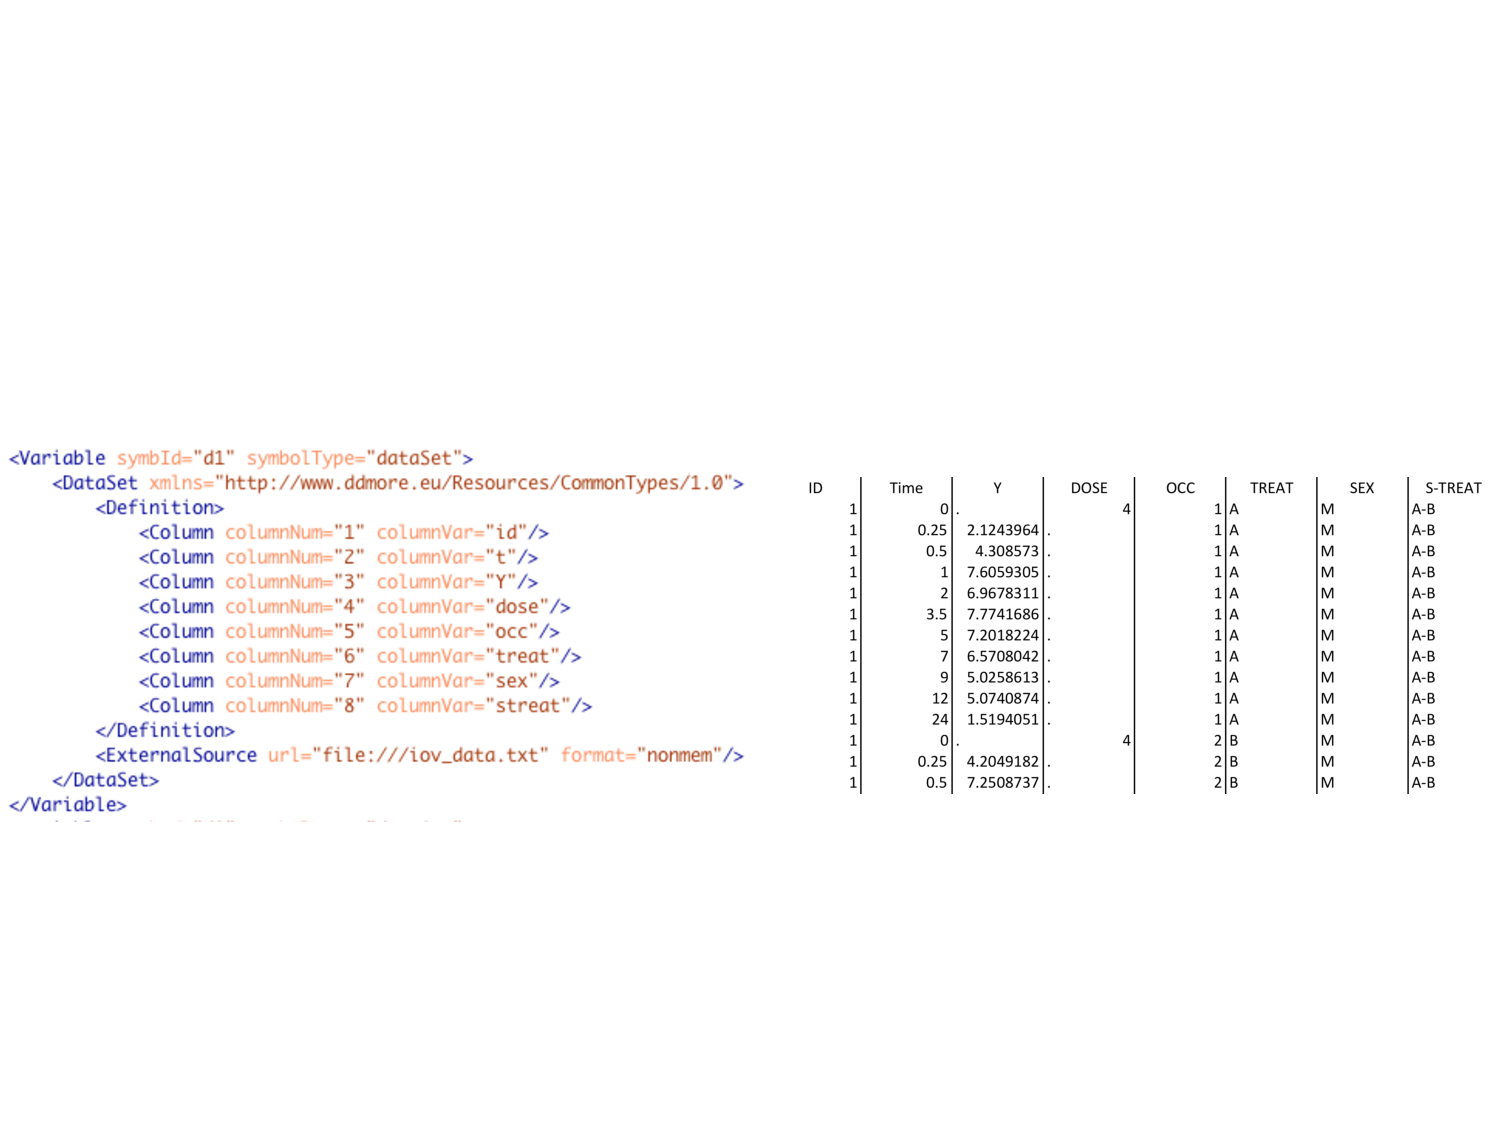
\includegraphics[width=\linewidth,clip=true,trim=0 5.2cm 0 7.5cm]{FirstDatasetExample}
%   \caption{An example of a dataset that corresponds to the contents
%     of a file on the right. Note how the column names in the file are
%     \emph{not} identical to those of the dataset definition. It is the
%     \xatt{columnNum} attribute that determines which column in the
%     file is mapped to which dataset column. }
%   \label{fig: dataset1-eg}
% \end{figure*}

As usual the simplest way to explain it is to look at an example, such
as the code snippet below:
%
\begin{xmlcode}
<ds:DataSet>
    <ds:Definition>
        <ds:Column columnId="id" valueType="string" columnNum="1"/>
        <ds:Column columnId="arm" valueType="string" columnNum="2"/>
        <ds:Column columnId="reps" valueType="int" columnNum="3"/>
    </ds:Definition>
    <ds:Table>
        <ds:Row>
            <ct:String>i1</ct:String><ct:String>a1</ct:String><ct:Int>20</ct:Int>
        </ds:Row>
        <ds:Row>
            <ct:String>i2</ct:String><ct:String>a2</ct:String><ct:Int>20</ct:Int>
        </ds:Row>
        <ds:Row>
            <ct:String>i3</ct:String><ct:String>a3</ct:String><ct:Int>40</ct:Int>
        </ds:Row>
        <ds:Row>
            <ct:String>i4</ct:String><ct:String>a4</ct:String><ct:Int>40</ct:Int>
        </ds:Row>
    </ds:Table>
</ds:DataSet>
\end{xmlcode}
%
As before the dataset has a definition, where the columns of the
dataset table are defined. The column number must start at 1 and each
column must be numbered in consecutive order (i.e.\xspace
1,2,3,4\ldots etc.). The type of each column is specified and this
complies with the \pharmml type system.  Next the content of the
dataset is held within the \xelem{Table} element and this consists of
one or more \xelem{Row} elements. Each row must contain an entry for
each column defined. NULL values are indicated by the \xelem{Null/}
element.

This looks like a table in a relational database and indeed this
approach is based on the concept of a relation in relational
theory. Therefore the ordering of rows is not significant. At present
there is no mechanism to define a key on the dataset or columns that
cannot be NULL. It is assumed that such restrictions may be applied when
the dataset is used. For example it is assumed that when mapping
observations in the \xelem{EstimationStep} none of the data is
NULL and that the combination of the time column and that identifying
the individual are unique.

\begin{figure}[htb]
\centering
%\setlength\fboxsep{0pt}
%\setlength\fboxrule{0.5pt}
%\fbox{%
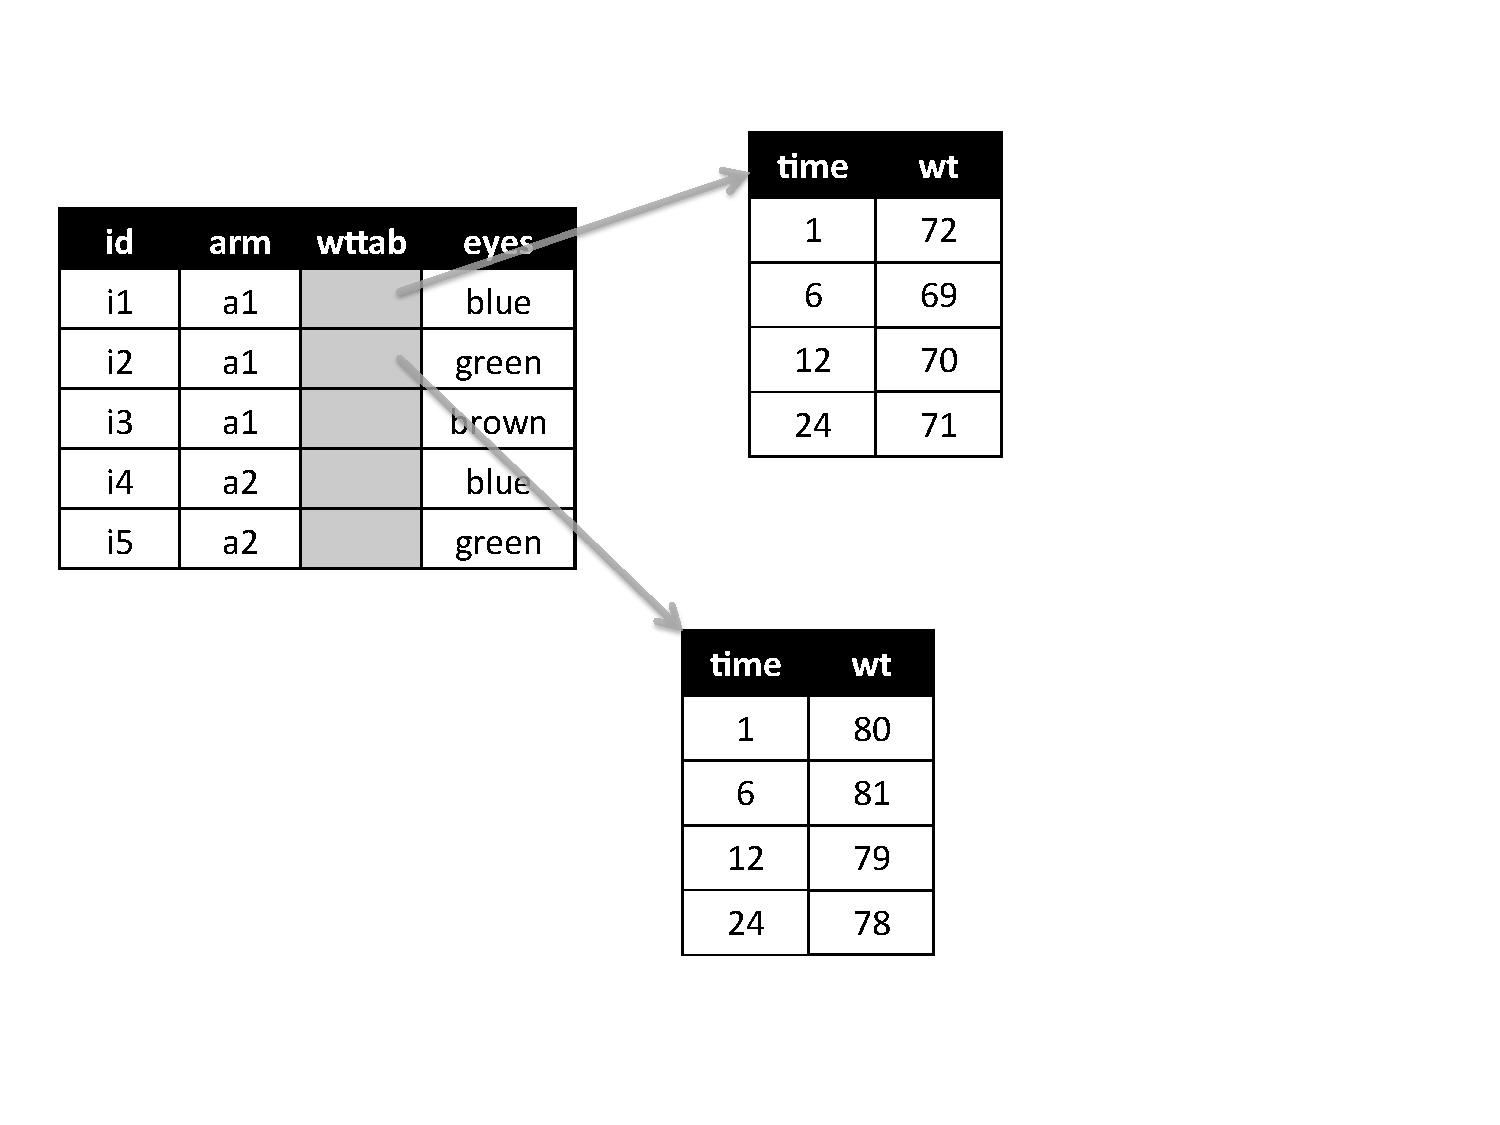
\includegraphics[height=0.35\textheight,clip=true,trim=9mm 1.5cm 8.3cm 2cm]{Datasets}%
%}
\caption{An illustration of how a table with a nested table can be
  conceptualised. Each cell within the \xatt{wttab} column contains
  another table.}
\label{fig:dataset}
\end{figure}

Finally, there is one deviation from standard relational theory in the
dataset. This is that a table can be nested multiple times, i.e., a
table can contain a column that defines another table and so on. This
concept is illustrated in figure \ref{fig:dataset}. We required this
because in some situations it is necessary to define one to many
relationships within the data. For example when defining a population
of individuals in a study whose weight changes during the course of
the study (weight is a time-dependent covariate). In relational theory
this is achieved by a foreign key relationship, but in the dataset it is
simpler and clearer if we take advantage of the hierarchical nature
of the XML. You can see this in the example dataset below:
%
\begin{xmlcode}
<ds:DataSet>
    <ds:Definition>
        <ds:Column columnId="id" valueType="string" columnNum="1"/>
        <ds:Column columnId="arm" valueType="string" columnNum="2"/>
        <ds:Table tableId="wttab" columnNum="3">
            <ds:Definition>
                <ds:Column columnId="time" valueType="real" columnNum="1"/>
                <ds:Column columnId="wt" valueType="real" columnNum="2"/>
            <ds:Definition>
        </ds:Table>
        <ds:Column columnId="eyes" valueType="string" columnNum="4"/>
    </ds:Definition>
    <ds:Table>
        <ds:Row>
            <ct:String>i1</ct:String><ct:String>a1</ct:String>
            <ds:Table>
                <ds:Row>
                    <ct:String>1</ct:String><ct:Real>72</ct:Real>
                </ds:Row>
                <ds:Row>
                    <ct:String>6</ct:String><ct:Real>69</ct:Real>
                </ds:Row>
                <ds:Row>
                    <ct:String>12</ct:String><ct:Real>70</ct:Real>
                </ds:Row>
                <ds:Row>
                    <ct:String>24</ct:String><ct:Real>71</ct:Real>
                </ds:Row>
            </ds:Table>
            <ct:String>blue</ct:String>
        </ds:Row>
        <ds:Row>
            <ct:String>i2</ct:String><ct:String>a1</ct:String>
            <ds:Table>
                <ds:Row>
                    <ct:String>1</ct:String><ct:Real>80</ct:Real>
                </ds:Row>
                <ds:Row>
                    <ct:String>6</ct:String><ct:Real>81</ct:Real>
                </ds:Row>
                <ds:Row>
                    <ct:String>12</ct:String><ct:Real>79</ct:Real>
                </ds:Row>
                <ds:Row>
                    <ct:String>24</ct:String><ct:Real>78</ct:Real>
                </ds:Row>
            </ds:Table>
            <ct:String>green</ct:String>
        </ds:Row>
    </ds:Table>
</ds:DataSet>
\end{xmlcode}
%
In the example the child table is defined by using a \xelem{Table}
element instead of the usual \xelem{Column} element and given the
identifier ``wttab''. Within the nested table definition another set
of columns is specified\footnote{Of course this definition can itself
contain another table definition \emph{ad infinitum}.}. Now when
encoding the data within the dataset its rows are defined as before,
but where a column has been replaced by a nested table the contents of
this table are delimited by a \xelem{Table} element. The dataset in
the example defines individual \texttt{i1} assigned to arm
\texttt{a1} with a weight that varies between $69$ kg and $72$ kg during
the study.

% in figure
% \ref{fig: dataset1-eg}. The \texttt{<DataSet>} element declares that
% what follows is a dataset and the \texttt{<Definition>} element
% defines the columns used by the dataset. Each column is defined by a
% number identifying the column (starting at 1) and is given a name
% (using the attribute \texttt{columnVar}). Both column number and
% column name must be unique within the dataset definition. Finally, the
% source of the dataset is defined. In this case the source is outside
% the \pharmml document (external) and is identified by a URL\@. The format
% of the external resource is also defined, in this case a file in
% \nonmem data format. The comma-separated and tab-delimited formats
% mentioned above are also available.

% \begin{listing*}[htb]
% \inputxml{dataset_internal.xml}
% \caption{Defining dataset data within \pharmml.}
% \label{code:dataset-internal-data}
% \end{listing*}

% In the example (\ref{fig: dataset1-eg}) the variable \attval{d1} is
% initialised with the data in the resource referenced by the
% \xelem{ExternalSource} element (in this case a file). It is important
% to note that unlike \nonmem the names given to each column of the
% dataset is \emph{not} significant. For example, calling a column
% \dscol{TIME} does not imply that this column contains time
% point data. This information is defined later by mapping the
% columns of a dataset to other parts of the \pharmml document
% (c.f.\ section \ref{sec:objective-data-mapping}).

% \begin{listing*}[htb]
% \inputxml{dataset_internal_ref.xml}
% \caption{Creating one dataset from another.}
% \label{code:dataset-internal-ref}
% \end{listing*}

% Data-sets do not need to be sourced from an external source. Their
% data content can be defined within the \pharmml document, as can be seen
% in listing \ref{code:dataset-internal-data}. This illustrates an
% additional concept not seen in the external data source a NULL value,
% encoded by the \xelem{Null} element, which means that no value has
% been provided or exists. This can also be defined by a special
% character in the external data source format, for example in \nonmem
% format the ``.'' indicates no value and so is for our purposes NULL.

% \begin{table}[htb]
% \centering
% \begin{tabular}{r r r r}\toprule
% ID & Time & Y & dose\\\midrule
% 1 & 0 & . & 4 \\
% 1 & 0 & . & 4 \\
% 2 & 0 & . & 4 \\
% 2 & 0 & . & 4 \\
% 3 & 0 & . & 4 \\
% 3 & 0 & . & 4 \\\bottomrule
% \end{tabular}
% \caption{The dataset obtained by selecting a subset of columns
%   from the original dataset and then eliminating all rows where
%   DOSE is NULL.}
%   \label{fig:restricted dataset}
% \end{table}

% A third way to define a dataset is to create it from another, as
% illustrated in listing \ref{code:dataset-internal-ref}. This allows
% you to choose a subset of the original dataset. As you can see this
% can be done in two ways: by selecting a subset of the columns from the
% original dataset or by choosing a subset of its rows based on some
% logical criteria (in \pharmml this is called a \emph{restriction}). In
% the example we are excluding all rows except those with a dosing value
% defined (i.e.\xspace where the column value is not NULL). This allows
% us to extract the dataset in figure \ref{fig:restricted dataset} from
% the original dataset shown in figure \ref{fig: dataset1-eg}.


\section{Mathematical expressions}
\label{sec:maths}
Mathematical expressions are a fundamental part of a pharmacometric
model and so it was important that \pharmml incorporated the
ability to encode these. The question we had in designing the language, however, was
what is the best way to do this?  Our initial approach was to reuse an
existing W3C standard called
\mathml\footnote{\url{http://www.w3.org/TR/MathML3/}}, which was
designed to represent mathematical equations on web pages.
Unfortunately, the full \mathml standard is bigger and more complex
than we need: indeed much of the standard focuses on the presentation
and layout of mathematical equations rather than their underlying
meaning\footnote{We should emphasise that his is not a criticism of
\mathml, as this was the problem it was created to solve!}.  This
was also the conclusion reached for similar standards to \pharmml such as
SBML \cite[Section 3.4]{sbmll3v1c},
CellML\footnote{\url{http://www.cellml.org/specifications/cellml_1.1/\#sec_mathematics}}
and \sedml \cite{sedmll1v1}. Their solution to this problem was to use
a subset of the standard that did what they wanted and to develop their
own software to support this subset. In effect they created their own
version of the \mathml standard. This means that the CellML version of
\mathml is not compatible with the \sbml version and so on, and as a
consequence each standard has had to develop its own software
libraries to support their own version of \mathml.

Faced with the same dilemma we considered adopting yet another subset
of \mathml, but decided against it for a number of reasons:
\begin{enumerate}
\item Because \mathml is designed for the presentation of maths its
  basic design is much more complicated than we require.
\item The design of \mathml is such that it is impossible to validate
  whether a sensible mathematical expression has been formed using
  just XML Schema validation\footnote{XML Schema is an XML standard
    that let's you effectively define an object model in XML. The
    benefit of the standard is that it there many tools that can then
    validated automatically whether your XML document conforms to this
    `object model'. We have taken advantage of this technology in
    \pharmml and it has made development of the specification and
    software support much more efficient.}. This is because it uses
  \verb|<apply></apply>| elements to group operands and operators
  together and so a statement such as
  \verb|<apply><divide/><cn>20/<cn></apply>| ($\div 20$) is
  syntactically valid \mathml, but an incomplete mathematical
  expression.
\item Taking a subset of \mathml requires the creation of a new XML
  Schema definition, new tools for validation and is effectively
  creating a new standard. In our view calling this \mathml is
  misleading as each of the \mathml subsets currently used are not the
  same and cannot be exchanged with each other, nor with W3C \mathml
  (see discussion above).
\end{enumerate}
Consequently we created our own mathematics definition, which has the
following design goals:
\begin{enumerate}
\item Have a design that ensured that mathematical expressions
  were syntactically correct --- allowing us to use XML Schema
  validating software to ensure this correctness.
\item Ensure that the maths could handle all mathematical expressions
  we require in \pharmml.
\item Provide logical expressions for use in piecewise functions.
\item Have a simple and concise design that could be easily written by hand
  and also read by a developer --- to facilitate testing.
\end{enumerate}

Our design follows that of many programming languages, such as C
\cite{Kernighan:1988:CPL:576122}, by defining unary and binary
operators that take one or two operands respectively. Such operands
can be literal values (e.g.\xspace numbers), variables or another
operator. In languages such as C, mathematical expressions are
designed to be easily read by humans, but in \pharmml we don't have
this restriction and we are more interested in ease of computational
processing. For this reason we have adopted a prefix representation.

%\begin{listing*}[htb]
% \inputxml{basic_maths_eg.xml}
% \caption{A simple equation encoded in \pharmml Maths. It
% is equivalent to the expression $(9 - 5) \times 2$.}
% \label{code:math-eg}
% \end{listing*}

In a prefix representation, also called Polish notation\footnote{For
  more information see
  \url{http://en.wikipedia.org/wiki/Polish_notation}.}, the operator is
placed before its operands. We can illustrate this using the following
expression, $(9 - 5) \times 2$, becomes $\times-9\,5\,2$. This is
evaluated from left to right. You first evaluate the operator which
has operands that are numerical values. The result of this operator is
then used as an operand of another operator and the process is
repeated until all operators are evaluated. Using the expression above
as an example: $-9\,5$ is evaluated first that then reduces the
expression to $\times 4\,2$, until finally we are left with the result
of $2$. The benefits for the parser are obvious because we no longer
require grouping constructs like parenthesis. As can be seen in the
following listing, this prefix approach fits well with XML and allows
us to express the above expression concisely\footnote{In fact the XML
  structure actually defines the abstract syntax tree of the
  mathematical expression, which is typically the output of a language
  parser.}.
%
\begin{xmlcode}
<!-- (9 - 5) * 2 -->
<Equation xmlns="http://www.pharmml.org/2013/03/Maths"/>
    <Binop op="times">
        <Binop op="minus">
            <ct:Real>9</ct:Real>
            <ct:Real>5</ct:Real>
        </Binop>
        <ct:Int>2</ct:Int>
    </Binop>
</Equation>
\end{xmlcode}
%
It also allows us to use XML Schema validation to ensure correctness
because we can validate that all binary operators require two operands
and a unary operator one. The more complicated example below shows how
to define the expression $\exp\left(-\textrm{logit}(i) + \beta
  \ln\left(\frac{W}{70}\right)+\eta\right)$ with unary and binary
operators:
\begin{xmlcode}
<?xml version="1.0" encoding="UTF-8"?>
<Equation xmlns="http://www.ddmore.eu/Resources/Maths/1.0"/>
    <!-- Omitted namespace declarations -->
    <Uniop op="exp">
        <Binop op="plus">
            <Uniop op="minus">
                <Uniop op="logit">
                    <ct:SymbRef symbIdRef="i"/>
                </Uniop>
            </Uniop>
            <Binop op="plus">
                <Binop op="times">
                    <ct:SymbRef symbIdRef="beta"/>
                    <Uniop op="ln">
                        <Binop op="divide">
                            <ct:SymbRef symbIdRef="W"/>
                            <ct:Real>70</ct:Real>
                        </Binop>
                    </Uniop>
                </Binop>
                <ct:SymbRef symbIdRef="eta"/>
            </Binop>
        </Binop>
    </Uniop>
</Equation>
\end{xmlcode}

Besides mathematical expressions \pharmml Maths can also define logical
expressions used in conditional logic that enables us to define
piecewise functions. %
% and these conditions can be used independently in
%the manner of an SQL WHERE clause (c.f.\xspace section
%\ref{sec:dataset}).
This uses the same postfix approach, but with alternate logical binary
and unary operators defined by the \xelem{LogicBinop} and
\xelem{LogicUniop} elements, respectively. The following example shows
how it can be combined with mathematical expressions to describe the
piecewise expression:
%
\[
\begin{cases}
-x & \text{if } x < 0\\
 x & \text{if } x \geq 0
\end{cases}
\]
%
Note that because logical expressions can contain strings it is
possible to define such expressions using non-numerical criteria:
%
\begin{xmlcode}
<Equation xmlns="http://www.ddmore.eu/Resources/Maths/1.0"/>
    <!-- Omitted namespace declarations -->
    <Piecewise>
        <Piece>
            <Uniop op="minus">
                <ct:SymbRef symbIdRef="x"/>
            </Uniop>
            <Condition>
                <LogicBinop op="lt">
                    <ct:SymbRef symbIdRef="x"/>
                    <ct:Int>0</ct:Int>
                </LogicBinop>
            </Condition>
        </Piece>
        <Piece>
            <ct:SymbRef symbIdRef="x"/>
            <Condition>
                <LogicBinop op="geq">
                    <ct:SymbRef symbIdRef="x"/>
                    <ct:Real>0</ct:Real>
                </LogicBinop>
            </Condition>
        </Piece>
    </Piecewise>
</Equation>
\end{xmlcode}

A complete list of the mathematical and operators that are available
is provided in section~\ref{sec:phmaths-defns}.  Here you will also
find a description of each operator's semantics and the permitted types
of its operands.

\section{Representing statistics}

As can be seen in chapter \ref{chap:mathsdefn}, \pharmml relies on the
ability to use probability distributions to describe the variability
in a pharmacometric model. Admittedly, the most commonly used
distribution is the normal distribution (or transformations of it),
but our intention is that \pharmml will have the flexibility to
describe a wide range of probability distribution types. To do this
the languages uses \uncertml version
3\footnote{\url{http://www.uncertml.org}}, which is an XML Schema
based language that aims to ``describe and exchange
uncertainty''. UncertML supports all the commonly used continuous and
discrete probability distributions and so more than adequately
supports the needs of \pharmml.  As an example we can show how the
normal distribution $\mathcal{N}(0, \omega^2)$ can be defined in
\uncertml.
% shown in listing \ref{code:normal-dist-eg}.
\begin{xmlcode}
<NormalDistribution xmlns="http://www.uncertml.org/3.0"
    definition="http://www.uncertml.org/distributions/normal">
    <mean><rVal>0</rVal></mean>
    <stddev><var varId="omega"/></stddev>
</NormalDistribution>
\end{xmlcode}

% \begin{listing*}[htb]
% \inputxml{normal.xml}
% \caption{XML code encoding the normal distribution, $\mathcal{N}(0,
%   1)$.}
% \label{code:normal-dist-eg}
% \end{listing*}


% \section{Representing the Structural Model}

% In \pharmml one of our aims has been to reuse existing standards where it
% makes sense to do so. One standard that is suited for this purpose is
% \sbml. It can be used to encode systems of ODEs or algebraic
% equations, but it can also encode more complicated mechanistic models
% too. For example models that describe signalling pathways spanning
% multiple compartment. Therefore, it is our preferred mechanism for
% representing the structural model in \pharmml.

% However, in order to use a structural model encoded in \sbml we need
% to somehow incorporate it into the \pharmml document. We do this with the
% \xelem{Import} element as can be seen in listing
% \ref{code:import-eg}. In doing so the import statement maps equivalent
% variables in the \pharmml document to those in the \sbml model.

% \begin{listing*}[htb]
% \inputxml {sbml-import1.xml}
% \caption{This snippet illustrates how we map the parameters
%   and variables in the \pharmml document to the \sbml model. The model
%   itself is identified by a URL and the type of model is identified as
% \attval{sbml}. The variables and the parameters (not shown) in the
% \pharmml document are mapped to those in the \sbml model.}
% \label{code:import-eg}
% \end{listing*}

% In addition to incorporating \sbml models we can also incorporate
% other structural models defined in \pharmml. This mechanism is there for
% completeness and is not the preferred method for including models,
% so we will not go into in more detail here.

\section{Time}
\label{sec:independent-var}

Time is required by most pharmacometric models and in \pharmml it can
be referred to explicitly. The symbol used for the time variable is
configurable at the beginning of the document as shown below:
%
\begin{xmlcode}
<PharmML xmlns="http://www.pharmml.org/2013/03/PharmML"
    xmlns:xsi="http://www.w3.org/2001/XMLSchema-instance"
    xsi:schemaLocation="http://www.pharmml.org/2013/03/PharmML ..."
    xmlns:math="http://www.pharmml.org/2013/03/Maths"
    xmlns:ct="http://www.pharmml.org/2013/03/CommonTypes"
    xmlns:ds="http://www.pharmml.org/2013/08/Dataset"
    xmlns:design="http://www.pharmml.org/2013/03/TrialDesign"
    writtenVersion="0.1">
    <ct:Name>IOV1 with covariates</ct:Name>
    <IndependentVariable symbId="t"/>
\end{xmlcode}
%
%(see listing \ref{code:indep-var-eg}).
Rather than time we call the element \xelem{IndependentVariable}
because this is more correct and because you could define a model that
uses another quantity than time as the independent variable (e.g.\xspace
dose in a dose-response model). Note that the independent variable
always has a real type.

% \begin{listing*}[htb]
% \inputxml{indep_var_eg.xml}
% \caption{{In this code snippet the independent variable is defined as $t$.}}
% \label{code:indep-var-eg}
% \end{listing*}

% \section{Units}
% \label{sec:units}

% \pharmml allows you to specify the units of the quantities in a
% model. This may seem like a trivial thing to do, but when such
% quantities are incorporated into equations (as they are here)
% then we need to take steps to ensure units are consistent with each
% other. That is, we need to check that the dimensions on the left hand side of an
% equation match those on the right and that the units have the same
% scale. For example it should recognised that $1000$ and $1kg$ are
% equivalent as are $0^o C$ and $32^o F$.

% The other issue is what units to support? Clearly the number of
% possible units is large and trying to predefine all possible units
% will be a cumbersome task. Instead we have borrowed the approach used
% by SBML \cite[Section 4.4]{sbmll3v1c} where units are defined using a
% set of basic units\footnote{Our approach varies slightly from that of
%   SBML in that we strick to a minimal set of base units and we allow
%   unit definitions to be built up from other unit definitions.}. These
% `built-in' units cover all dimensions and can be used to build up any
% specific unit. For example we may have a $g$ as the fundamental unit
% of mass and then define a $kg$ which is a gram scaled by 1000. An
% example of what it might look like is below:
% %
% \begin{xmlcode}
% <UnitDefinition symbId="hour">
%     <Symbol>h</Symbol>
%     <Unit basicUnit="second">
%         <Exponent>1</Exponent>
%         <Scale>0</Scale>
%         <Multiplier>3660</Multiplier>
%     </Unit>
% </UnitDefinition>
% \end{xmlcode}
% %
% As you can see, the \xelem{UnitDefinition} element defines the unit in
% terms of a base unit referred to in the \xelem{Unit} element.  The
% \xelem{Unit} element describes the conversion of the base unit a
% consistent of the unit being defined. This defines the unit
% $mathit{hour}$ as $(3660 \cdot 10^0 \cdot \mathit{second})^1$: in
% otherwords 1 hour is 3600 seconds.  The base units used in \pharmml
% are the seven base units from SI\footnote{See Section 2 in
%   \url{http://http://www.bipm.org/utils/common/pdf/si_brochure_8.pdf}.}
% plus a dimensionless unit (see section~\ref{sec:base-units-defn}). The
% components of the definition are then combined in the following
% equation:
% %
% \[
% \mathit{unit} = \left(\mathit{multiplier} \cdot 10^{\mathit{scale}}
%     \cdot \mathit{baseunit} \right) ^{\mathit{exponent}}
% \]
% %
% More complex units can contain multiple \xelem{Unit} elements:
% %
% \begin{xmlcode}
% <UnitDefinition symbId="velocity">
%     <ct:Symbol>ms-1</ct:Symbol>
%     <Unit basicUnit="metre">
%         <Exponent>1</Exponent>
%     </Unit>
%     <Unit basicUnit="second">
%         <Exponent>-1</Exponent>
%     </Unit>
% </UnitDefinition>
% \end{xmlcode}

% Combining unit definitions effectively multiplies then so above we
% define velocity as $ms^{-1}$. Note that if the \xelem{Scale} and
% \xelem{Multiplier} elements are omitted they are assumed to be 0 and 1
% respectively. The example below shows how we might use these
% definitions, for example to define the time units used in the model:
% %
% \begin{xmlcode}
% <IndependentVariable symbId="t">
%     <Units symbId="hour"/>
% </IndependentVariable>
% \end{xmlcode}

% Note also that derived units can be composed from other derived
% units as shown below, where the unit $mg$ is first derived from the
% base unit kilogram as $(1 \cdot 10^-3 \cdot kg)^1$ and the unit $mg/kg$ is
% derived as a combination of $(1 \cdot 10^0 \cdot kg)^-1$ and $(1
% \cdot 10^0 \cdot kg)^1$.
% \begin{xmlcode}
% <ct:UnitDefinition unitId="mg">
%     <ct:UnitComponent>
%         <ct:BasicUnitRef basicUnit="kilogram"/>
%         <ct:Exponent>1</ct:Exponent>
%         <ct:Scale>-4</ct:Scale>
%     </ct:UnitComponent>
% </ct:UnitDefinition>
% <ct:UnitDefinition unitId="mg_kg-1">
%     <ct:UnitComponent>
%         <ct:UnitRef unitId="mg"/>
%     </ct:UnitComponent>
%     <ct:UnitComponent>
%         <ct:BasicUnitRef basicUnit="kilogram"/>
%         <ct:Exponent>-1</ct:Exponent>
%     </ct:UnitComponent>
% </ct:UnitDefinition>
% \end{xmlcode}

% In this version of \pharmml unit definitions are optional and unit
% consistency is not be enforced. In other words there is no validation
% rule stating that units must be consistent. The aim is to first
% establish the structures to define units within the specification and
% then at a future date to add rules about unit consistency. Why not
% now? Largely pragmatism. Unit consistency can only be enforced if all
% quantities in the \pharmml document use them, so to make such
% consistency mandatory will put a burden on tool developers. We would
% prefer to defer this decision until we have all gained experience using
% units in \pharmml.

\section{Element identifier}
\label{sec:element-id}

We know that other resources will wish to interact with \pharmml and
so we have given some thought to how best they should refer to
specific pieces of information in a \pharmml document. Our solution is
to provide every XML element in the document with an optional unique
identifier. The listing below shows how the \xatt{id} attribute is
used:
%
\begin{xmlcode}
<FixedEffect id="e10" symbId="beta_V">
    <Covariate>
        <ct:SymbRef  symbIdRef="W"/>
    </Covariate>
</FixedEffect>
<FixedEffect id="e13" symbIdRef="beta_Cl">
    <Covariate>
        <ct:SymbRef symbIdRef="W"/>
    </Covariate>
</FixedEffect>
<RandomVariable id="e16" symbId="eta_V">
    <ct:VariabilityReference id="e17">
        <ct:SymbRef id="e18"  blkIdRef="model" symbIdRef="level"/>
   </ct:VariabilityReference>
   <!-- Snip -->
</RandomVariable>
\end{xmlcode}
%
As you can see the \xatt{id} attribute is optional and need only be
used for elements that you want to refer to. There are no rules other
than that the identifier must be unique within the \pharmml document.
Thus to refer to a specific part of a document all you need to define is
the location of the document and the identifier. So assuming that the
above code snippet is found in a file called ``testFile.xml'' a
suitable (relative) URI that refers to the random variable in the
example might be \url{testFile.xml#e16}.

The benefit of this approach is that the \xatt{id} attribute can
easily be made available programmatically and searched on with a class
library generated from the XML Schema.
%\footnote{We considered using the XPath
% standard\cite{xpath} to identify elements using what is in effect an
% XMl query language, but we felt that it would be very difficult to
% execute such queries on a class library encode in a programming
% language the query is on the XML not attributed help within the prograsuch as
% Java, which is what you would need to do when interacting with
% \pharmml via the libPharmML API (see section
% \ref{sec:libpharmml}).
This mechanism is also used successfully by SBML \cite[Section
6]{sbmll3v1c}. You will see in the sections below (sections \ref{sec:annotation} and
\ref{sec:extension}) how we take advantage of this mechanism to
annotate and extend a \pharmml document.

\section{Ordering modelling steps}

Descriptions in a modelling step are declarative, describing what
was done, what algorithms were used and what their properties were.

\begin{figure}[htb]
 \centering
  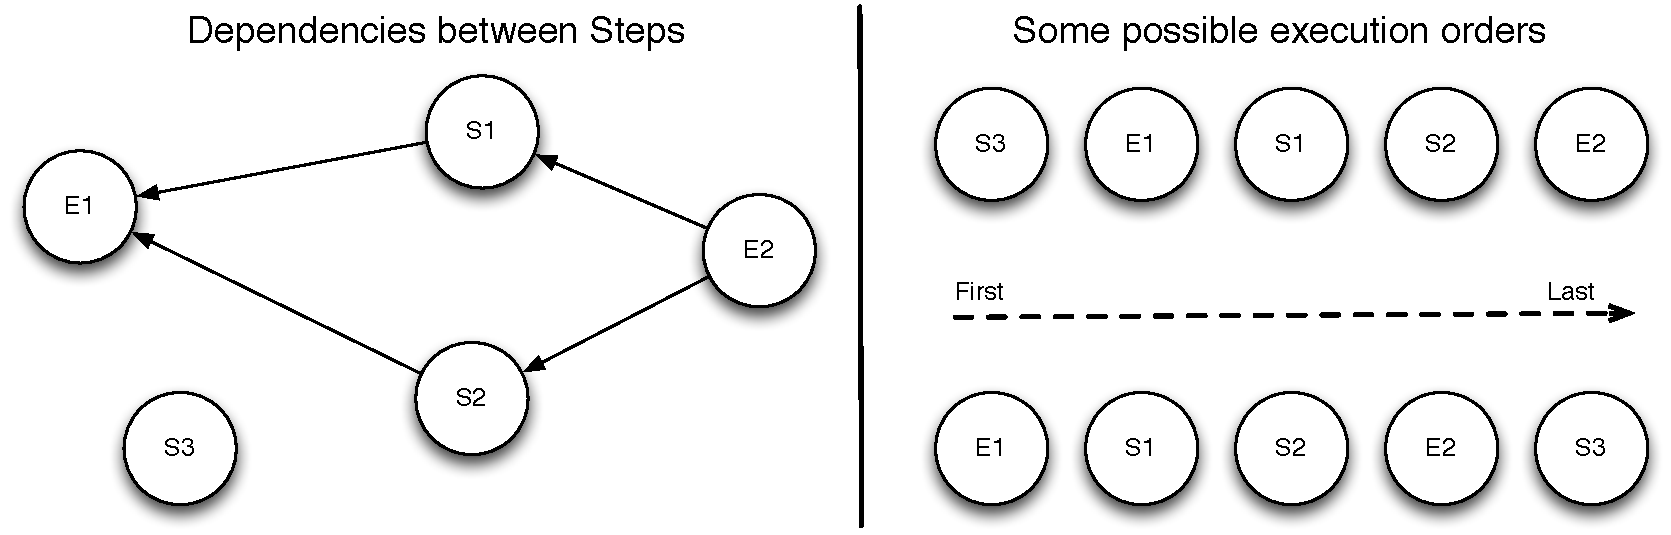
\includegraphics[width=1\linewidth]{ModellingStepDeps}
  \caption{An example of the dependencies between modelling steps is
    shown on the left. The arrow indicates the direction of the
    dependency so step S1 is dependent on the successful completion of
    step E1. So in this example step E1 must be executed before step
    S1 and S2, and those steps must both execute before step E2. On
    the right-hand figure we show two possible execution orders that
    correspond to the task dependecies on the left. It is important to
    remember that, as in this example, there can be more than one
    execution order for a given set of task dependencies.}
  \label{fig:modellingstep_deps}
\end{figure}

The \phsec{Modelling Steps} section has two components that describe
simulation or estimation tasks. Multiple tasks can be linked together so
that a given estimation task can be placed before a given simulation
task or no order can be given in which case tasks can be executed in
parallel or in any order. A task is ordered by defining its dependent
tasks: tasks that must complete successfully before it can start (see
figure~\ref{fig:modellingstep_deps}). In this way the modelling steps
make no assumptions about how or where its tasks are executed, but
provides enough information for a workflow engine to parallelise the
execution of its tasks successfully, should it wish to.

At the moment tasks cannot specify how output is generated from either
an Estimation or Simulation step. A result of this restriction is that
it is \emph{not} possible to exchange information from one modelling
step to another: for example to use the output of an estimation to set
the parameter values in an estimation. We recognise that this is a
limitation of the current version and this functionality will be
provided in a future release of \pharmml.


\section{Supporting Resources}
\label{sec:supporting-res}

\subsection{Metadata: annotating the \pharmml document}
\label{sec:annotation}

As has been stated above (Chapter \ref{chap:scope}), the purpose of
the \pharmml document is to provide a mathematical and structural
description of a pharmacometric model, sufficient for it to be
executed. Additional information, such as a description of the disease
process being modelled, the exact estimation algorithm or a
publication describing the model is not included in the \pharmml
document. Typically called metadata,
%\footnote{Metadata mean data about
  % data and is correctly used when referring to data that defines other
  % data: such as the definition of a relational database schema. In
  % this field metadata is the commonly used term for what may be more
  % accurately called annotation. However in the specification we have
  % followed convention and use the term metadata in this context.},
this information is still very important and so \pharmml aims to
provide support for external annotation.

\begin{figure}[htbp]
\centering
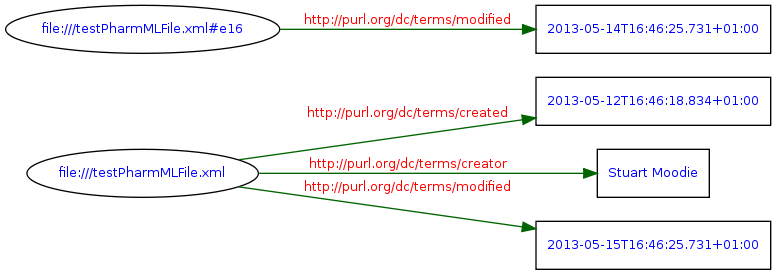
\includegraphics[width=0.8\linewidth]{rdf_graph}
\caption{This figure illustrates how information in the RDF example is
organised. Simply put the subject of the annotation is on the left and
is annotated by the object on the right. The meaning of that
annotation is described by the \emph{predicate} term labelling the
arrow. So reading the top subject from left to right we understand that
element \emph{e16} was \emph{modified} at \emph{14/05/13 at 4:46pm}.}
\label{fig:rdf-graph}
\end{figure}

We expect such metadata to take the form of ontological annotation and
while the detail of what will be annotated is out of scope of this
document we can show how this can work using a standard for describing
resources (such as XML documents) called Dublin Core\footnote{For more
  information see \url{dublincore.org}.}. Using this ontology we can
describe many things about a \pharmml document such as when and by
whom it was created or last updated. Typically such annotation is
expressed using a standard called RDF\footnote{See RDF URL}, which can
be updated and queried using associated software libraries. The
following example\footnote{This example is available as part of the
  examples provided with this specification at
  \texttt{examples/\-CombineArchive/\-annotation.xml}.} gives you a
flavour of what an RDF annotation of a \pharmml document would look
like if we were referring to the code snippet in
section~\ref{sec:element-id}.
%
\begin{xmlcode}
<rdf:RDF
    xmlns:rdf="http://www.w3.org/1999/02/22-rdf-syntax-ns#"
    xmlns:dcterms="http://purl.org/dc/terms/">
  <rdf:Description rdf:about="testPharmMLFile.xml">
    <dcterms:created>2013-05-12T16:46:18.834+01:00</dcterms:created>
    <dcterms:creator>Stuart Moodie</dcterms:creator>
    <dcterms:modified>2013-05-15T16:46:25.731+01:00</dcterms:modified>
  </rdf:Description>
  <rdf:Description rdf:about="testPharmMLFile.xml#e16">
    <dcterms:modified>2013-05-14T16:46:25.731+01:00</dcterms:modified>
  </rdf:Description>
</rdf:RDF>
\end{xmlcode}
%
The metadata above is encoded in RDF-XML\footnote{See \url{rdf-xml}}
and annotates two things. The first \xelem{rdf:Descr\-iption}
element states when the file was both created and modified and also
who created it. The second \xelem{rdf:Description} element points to
the XML element in the PharmML document with an \xatt{id} value of
``e16''. In the example in section \ref{sec:element-id} this is the
\xelem{RandomVariable} element and so we can deduce that this
description is telling us when this element was modified.
Another way of looking at RDF information is shown in figure
\ref{fig:rdf-graph}, which hopefully makes the relationships described
above even clearer. Of course this is a trivial example, but it
illustrates how the \pharmml document can be annotated using metadata
described in a separate RDF document.


\subsection{Standard Structural Models}

In many, if not the majority, of pharmacometric models the structural
model is selected from a standard library. Modelling tools such as
\nonmem or \monolix provide large platform specific libraries
\cite{NONMEM:2006aa} \cite{Bertrand:2008}. These have the benefit of
being both reusable and optimised to run efficiently on their target
platform. With \pharmml we want to support both of these features and
so we will be establishing a framework that provides the following:
\begin{description}
\item[a model ontology] an ontology describing all the models held in
  the standard library.
\item[tool specific mappings] using the model ontology this will
  provide mapping from the models in the standard library to tool
  specific models.
\end{description}

\begin{figure}[htb]
\centering
  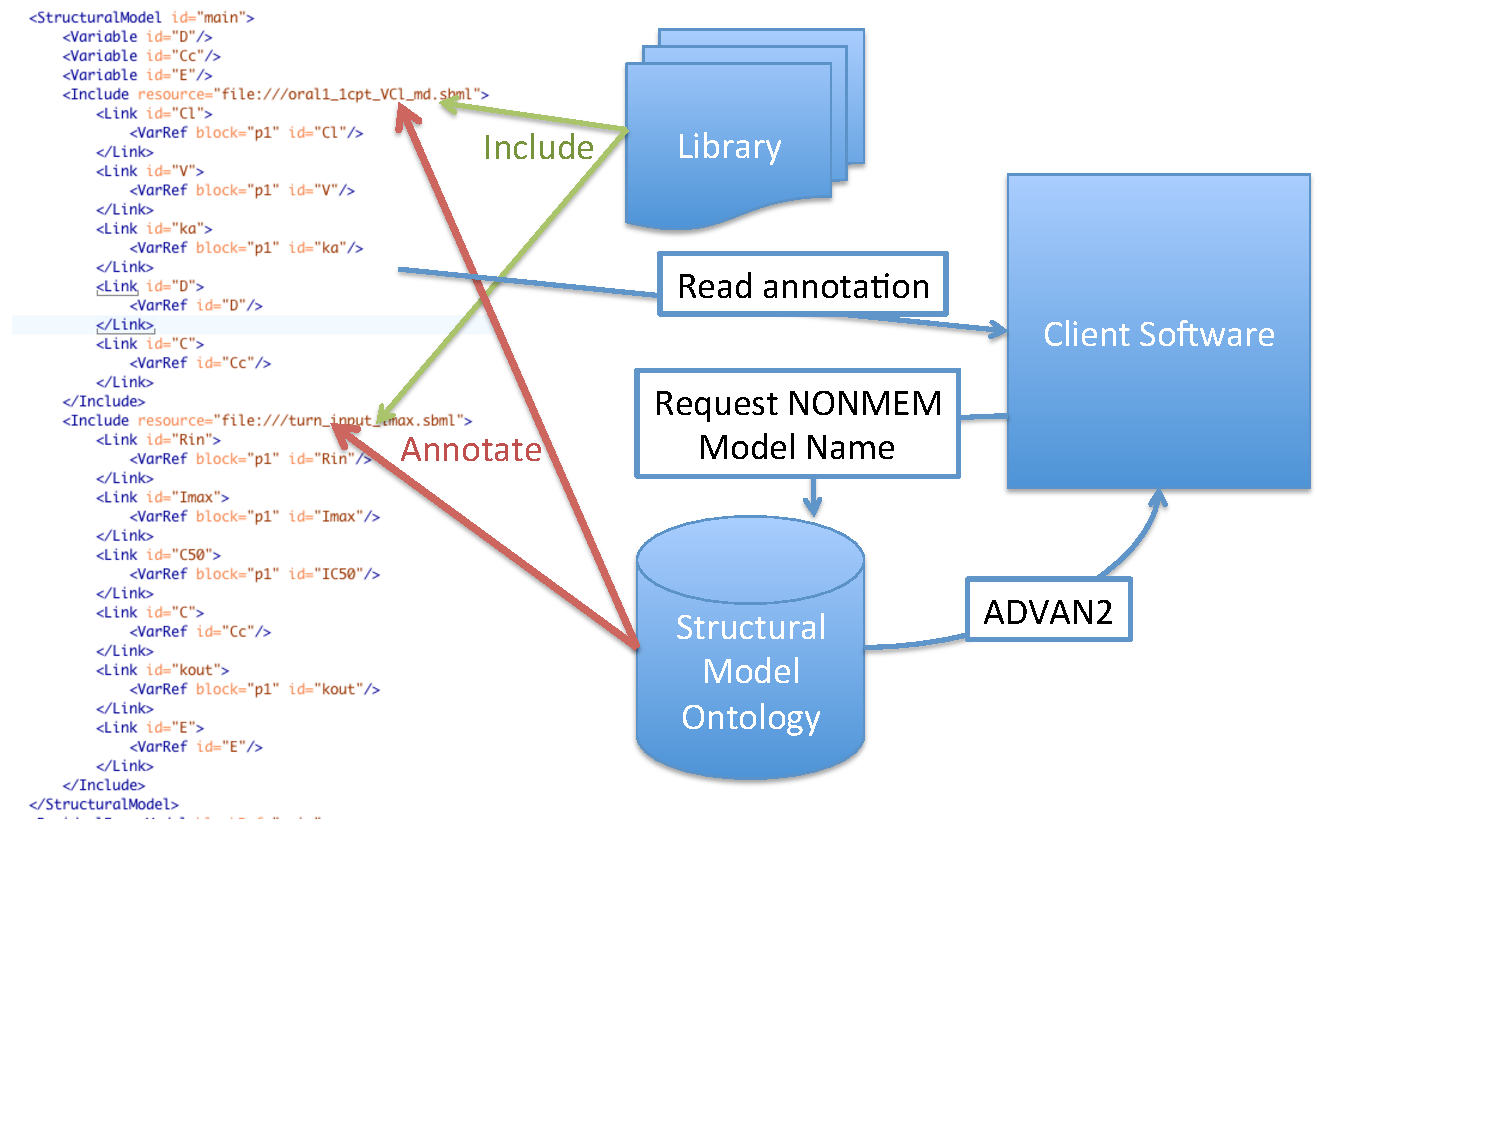
\includegraphics[width=0.9\linewidth,clip=true,trim=0cm 5.5cm 3.5cm 0cm]{ModelMapping}
  \caption{A schematic diagram illustrating how the standard library
    ontology framework is used to generate target specific code when
    translating \pharmml for a specific M\&S tool.}
  \label{fig:model-mapping}
\end{figure}

We expect that the structural model within the \pharmml document will
be annotated with the correct structural model using the model
ontology (following the annotation mechanism described above in
section~\ref{sec:annotation}).  The model ontology term can be used to
identify the appropriate model name for a given modelling tool by
using one of the tool-specific mappings. This allows \pharmml to
provide a tool-independent description of standard structural models.
It also allows conversion tools to convert a \pharmml model into a
tool specific encoding that takes advantage of its built-in structural
model library. This process is summarised in
figure~\ref{fig:model-mapping}.

\subsection{Extending PharmML}
\label{sec:extension}

As with any standard there will be circumstances when it does not
represent all the information that you would like and it would be
convenient to extend it. Typically there are two scenarios where this
is likely to be the case. The first is when the information is genuinely
not supported by \pharmml. This may be because it has not been
implemented yet, or it may be that there is no consensus about whether
this information should be included or no agreement about the best way
to represent it. The second scenario is when you want to
add application specific information to a \pharmml document. Perhaps
because a tool wishes to use \pharmml as its native storage format in
which case it would also want to store information about application
settings etc.

Whatever the reason \pharmml can be extended. Like the metadata
descriptions above (section \ref{sec:annotation}) this approach relies
on the element identifier (see section~\ref{sec:element-id}). The
recommended approach is that you develop a separate XML document
(typically in a separate file), which we will call the extension
document, using any XML representation you choose. Where information
in the extension document relates to the content of the \pharmml
document then you can refer to the relevant XML element using its
identifier.

\begin{figure}[htb]
\centering
  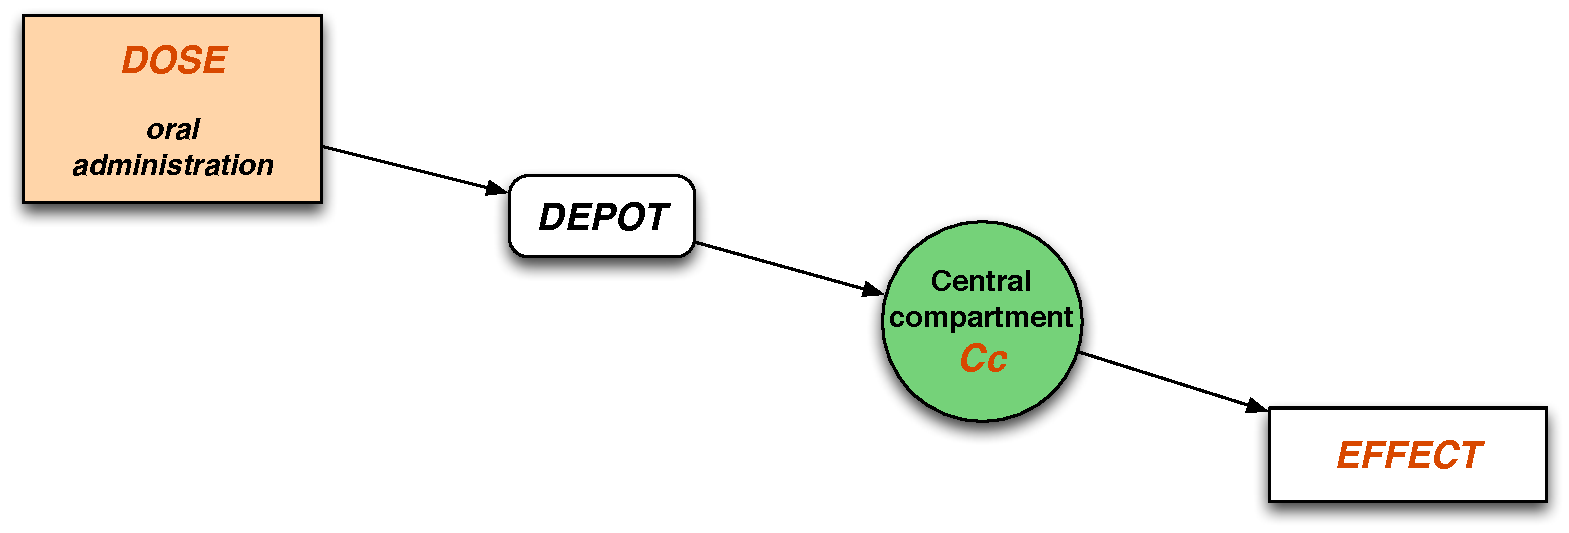
\includegraphics[height=0.2\textheight]{GraphicalModel}
  \caption{This diagram is reproduced from an example in the Monolix
    user manual \cite{Monolix4.1.4UserGuide:2012} and it provides a
    graphical description of a structural model. In the hypothetical
    example in the text we illustrate how you might extend \pharmml to
    link this graphic with the components of the model it represents.}
\label{fig:graphical-model}
\end{figure}

We can illustrate with an example based on the second scenario we
described above: application specific extensions. In this scenario our
software tool provides a graphical interface that lets you create a
pharmacometric model by drawing and connecting shapes such as the
diagram in figure~\ref{fig:graphical-model}. When you save the diagram
the application saves both the \pharmml that encodes the model and an
extension document that describes the graphical layout and maps the
graphical elements to the relevant parts of the model. The extension
document could look like this:
%
\begin{xmlcode}
<?xml version="1.0" encoding="UTF-8"?>
<Diagram resource="file:///anotherPharmMLFile.xml">
    <Rectangle id="1">
        <Name>Dose</Name>
        <Bounds x="10" y="10" w="50" h="30"/>
        <!-- Omitted other information such as colour and other text-->
        <Ref idRef="e35"/>
    </Rectangle>
    <!-- Omitted -->
    <Circle id="3">
        <Name>Central</Name>
        <Bounds x="10" y="200" w="45" h="45"/>
        <!-- Omitted other information such as colour and other text-->
        <Ref idRef="e46"/>
    </Circle>
    <!-- Omitted other shape definitions-->
    <Link src="1" tgt="2"/>
    <Link src="2" tgt="3"/>
    <Link src="3" tgt="4"/>
</Diagram>
\end{xmlcode}
%
The XML describes the shapes of the nodes, their location and the
connections between them. What allows it to extend the \pharmml document?
First the \xatt{resource} attribute provides a URL describing
the location of the \pharmml document being extended. Next the
\xelem{Ref} element defines a reference that points to an element in
the \pharmml document. From this information the application is able
to read both the \pharmml and the extension documents and then relate
the diagram to the relevant part of the model.

Note that while this is a hypothetical example for \pharmml, this type
of solution has been implemented by a graphical Systems Biology editor
called CellDesigner\footnote{\url{www.celldesigner.org}}. It uses SBML
as its native application format: encoding the model in SBML and using
SBML's extension facilities to store graphical information and other
application specific properties.

One final clarification. The extension mechanism does not require an
application to use the same XML elements as described in the example
above. The XML content of the extension document is entirely the
concern of the application. In order to extend a \pharmml document
all it must do is:
\begin{enumerate}
\item Specify how to find the \pharmml document. Using a URI is a good
  way to do this.
\item Use the element identifier to refer to the content of the \pharmml document.
\end{enumerate}

\subsection{Organising \pharmml resources}
\label{sec:pharmml-archive}

We expect that \pharmml will in normal usage consist of more than one
file. From the discussion about annotating
(section~\ref{sec:annotation}) and extending
(section~\ref{sec:extension}) \pharmml it is clear that both of these
cases require the creation of resources that are closely
related to a \pharmml document. It is therefore desirable that they
are kept together and exchanged and used together.

\begin{figure}[htb]
\centering
  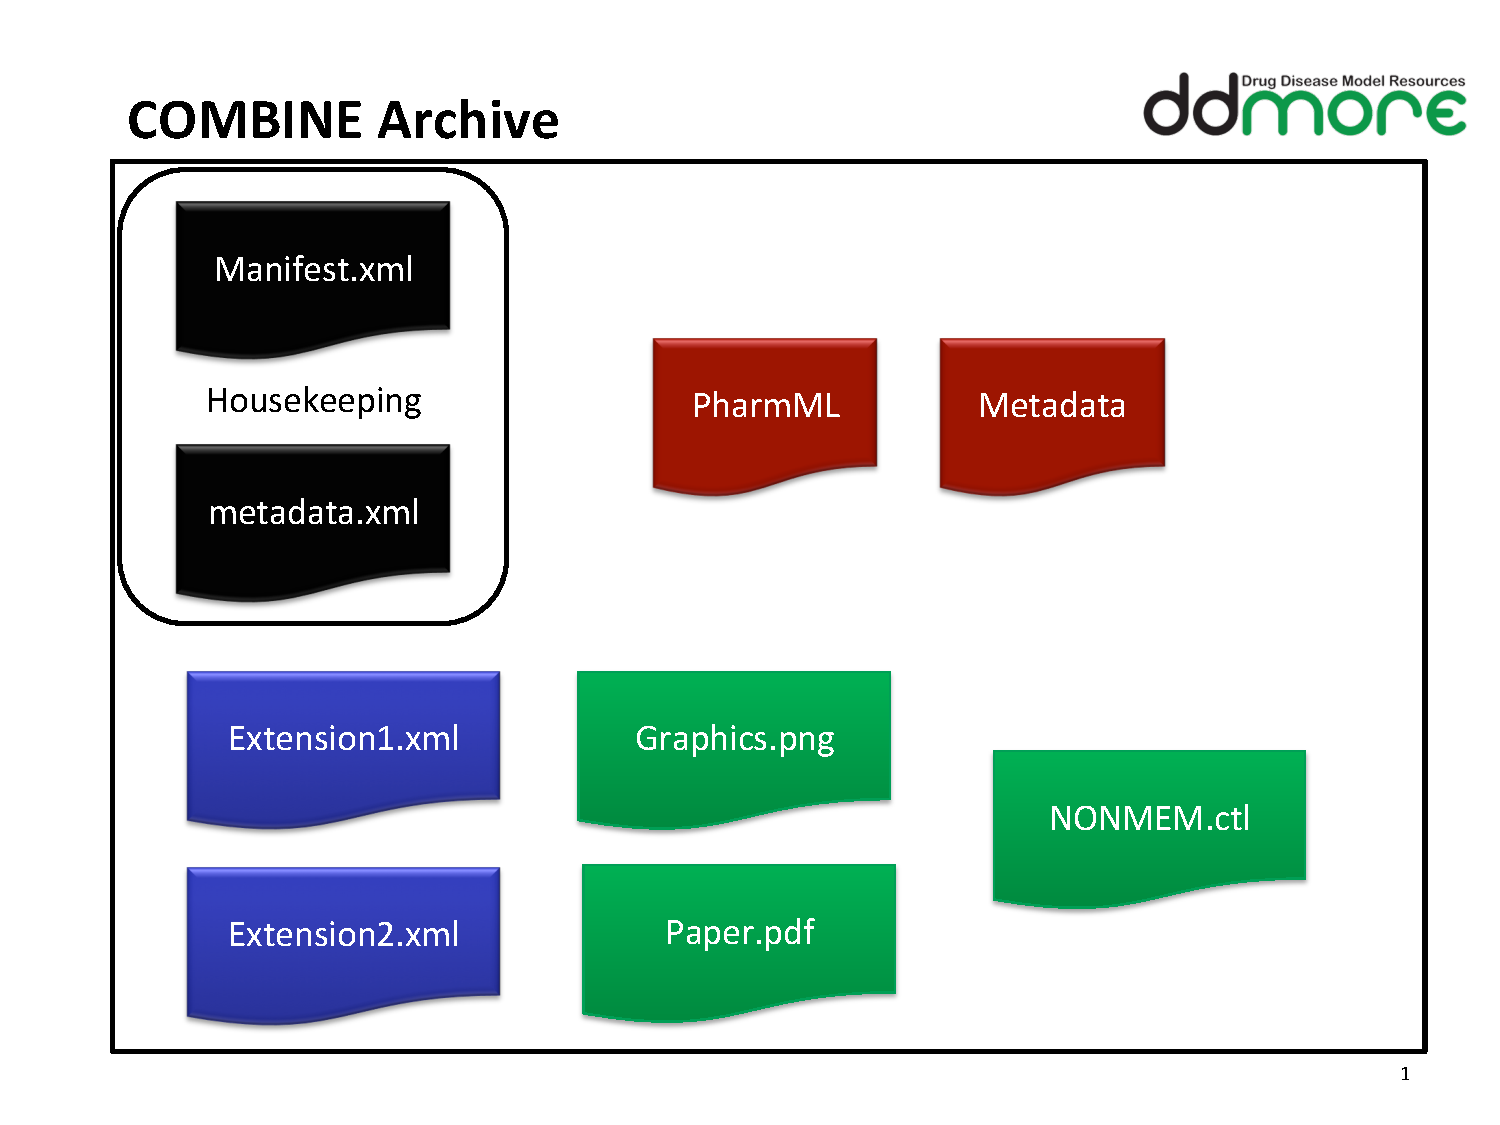
\includegraphics[width=0.6\textwidth]{AchiveOverview}
  \caption{An overview of how a COMBINE archive may be used to hold
    XML documents and files associated with a model encoded in
    \pharmml. In this example the archive holds the model and its
    metadata (in red) and two application specific extension
    documents (in blue). This also shows another advantage of using
    the archive: you can store other useful information, such as the
    original model file, relevant papers or images (in
    green). Finally, the archive contains a metadata file (in black)
    that helps an application reading the archive make sense of what
    it contains.}
  \label{fig:moml-archive-overview}
\end{figure}

An archive file can provide this functionality. It acts as a
container, and since it is a file can be easily exchanged and
stored. We recommend that you use an archive based on the emerging
COMBINE Archive
standard\footnote{\url{http://co.mbine.org/documents/archive}}. It is
based on a zip archive and holds additional information that allows
you to identify the modelling resources in the file. The exact details
of how it works is outside the scope of this document, but the
components of the archive and how it can be used to hold \pharmml
related resources is illustrated in
figure~\ref{fig:moml-archive-overview}\footnote{An example of a
  CombineArchive file that contains a metadata file annotating a
  \pharmml document can be found in \texttt{examples/CombineArchive/archive.zip}.}.

\subsection{Software support for \pharmml}
\label{sec:libpharmml}

\pharmml is a complex language. It is designed using an industry
standard, XML Schema\footnote{\url{http://www.w3.org/XML/Schema}}, which gives us the
ability to use widely available software packages to verify that the
XML file is correctly written and that elements are put in the right
place (syntax checking). However, \pharmml describes a pharmacometric
model and so there is a lot of information that is very specific to
this domain and cannot be validated by standard tools.  That's why we need
\pharmml specific software tools and libraries. Without such software
the burden of validation falls on the modelling tools reading and
writing \pharmml. Given the complexity of \pharmml's validation rules
it is unlikely that such validation would be complete and implemented
consistently, which makes our goal of exchange between modelling
tools less likely to succeed.

Therefore in parallel to the development of this specification a
software library called libPharmML\footnote{For more information see
  the libPharmML specification in the DDMoRe Interface Europe
  document repository: WP2 deliverables: \emph{D2.2
    libPharmMLTechSpec}.} is being developed to support it.  This will
allow you do the following:
%
\begin{enumerate}
\item Create a new \pharmml document.
\item Read an existing \pharmml document from a file (or other
  resource).
\item Write a \pharmml document to a file (or resource).
\item Validate that a \pharmml document complies with the XML Schema
  definition and the rules set out in this specification.
\end{enumerate}
%
The library is implemented in Java. There are no plans to implement an equivalent
version in another programming language, such as C++, but this could be done if
there was sufficient demand for it and sufficient developer resources were available
to implement it.
